\section{Differentials and Coordinate Transformations of Finite Elements}

For the following exposition we refer to~\cite{ciarlet},
 Section 3.9 of~\cite{monk} and~\cite{gh99}.

We want this same setting to build Finite Elements on 
arbitrary contiguous prisms
belonging to a fixed mesh, all of which being an affine 
image of the reference prism.
In order to do so we transform the set $\hat{E}$, the 
discrete local space and the 
degrees of freedom.

%===============
%exactly as we are told by the 
%push-forward
%transformations~(\ref{push-forward}). 
%===============

Consider the application $\hat{\bx}\longmapsto{\bx} = 
F_E(\hat{\bx})$, where $F_E = M_E\hat{\bx} + \bx_0$, that transforms
$\hat{E}$ in an element $E$ of the mesh and $M_E$ is invertible.

A scalar function $\hat{p} \in H^1(\hat{E})$ is transformed into a 
scalar function $p$ on $E$ with
\begin{IEEEeqnarray}{rCl}
    \label{transfEscalar} p\circ F_E & = & \hat{p}.
\end{IEEEeqnarray}
As it holds~(\cite{ciarlet})
\begin{IEEEeqnarray}{rCl} \label{aux_label4}
  \nabla p = M^{-t}\hat{\nabla} \hat{p} \circ F_K^{-1}\mbox{,}
\end{IEEEeqnarray}
then it results 
$p \in H^1(K)$. Gradients are taken with respect to the local coordinates
of $E$ and $\hat{E}$ in each case. The same will apply for every finite element
and for $\dv$ and $\curl$.

Now let $\hat{\bu} \in H(\curl, \hat{E})$. We want to assign to it a function
$\bu$ on $E$. As for $\hat{p}$ and $p$ as before it holds
$\nabla p \in H(\curl, E)$ and $\hat{\nabla} \hat{p} \in H(\curl, \hat{E})$,
equality~(\ref{aux_label4}) suggests the following transformation.
\begin{IEEEeqnarray}{rCl}
    \label{transfHcurl} \bu\circ F_E & = & M_E^{-t}\hat{\bu}.
\end{IEEEeqnarray} 
With this definition we have $\bu\in H(\curl, E)$ and also
\begin{IEEEeqnarray}{rCl}
    \label{transfCurl} (\textbf{curl}\,\bu)\circ F_K & = & 
    \frac{1}{\det M} M (\hat{\textbf{curl}}\,\hat{\bu})\mbox{,}
\end{IEEEeqnarray}
(cfr. Lemma 3.57, page 77 and Corollary 3.58 in~\cite{monk}).
Now we proceed in a similar way for $H(\dv)$. The relation 
$\hat\bu\in H(\curl,\hat E)$ implies $\curl\hat\bu\in H(\dv, \hat E)$
so~(\ref{transfCurl}) shows that to transform $\hat\bu\in H(\dv,\hat E)$
into $\bu\in H(\dv,E)$ we must do it via
\begin{IEEEeqnarray}{rCl}\label{transfDiv}
	\bu\circ F_E & = & \frac{1}{\det M_E}M_E\hat\bu.
\end{IEEEeqnarray}
By Lemma 3.59 in~\cite{monk}, if $\bu$ and $\hat\bu$ are related
by~(\ref{transfDiv}), then $\dv\,\bu = (\det M_E)^{-1}\dv\,\hat\bu$
and hence $\bu\in H(\dv,E)$ if and only if $\hat\bu\in H(\dv,\hat E)$.\\


**********************************************\\
Since $F_K$ is affine
\begin{IEEEeqnarray}{rCl}
    \label{transfDiv} \bu\circ F_K & = & 
    \frac{1}{\det M} M \hat{\bu}.
\end{IEEEeqnarray}


Then, with multiindex notation, for $F_K = \diag{h_1}{h_2}{h_3}$:
\begin{IEEEeqnarray*}{rCl}
    \partial^\alpha \hat{u} (\hat{\bx})&=&
        h^\alpha\partial^\alpha u(F_K(\hat{\bx})).
\end{IEEEeqnarray*}



With~(\ref{transfDiv})
\begin{IEEEeqnarray*}{rCl}
    \|\hat{\textbf{v}}\|^2_{L^2(\hat{E})}
    &=& \sum_{1\leqslant i\leqslant 3}\|\hat{v}_i\|^2_{0,\hat{E}}\\[7pt]
    &=& \sum_{1\leqslant i\leqslant 3}\frac{h_jh_k}{h_i}\,\|v_i\|^2_{0,K};\\[7pt]
    \|\hat{v}_i\|^2_{0,\hat{E}}&=&\frac{h_jh_k}{h_i}\,\|v_i\|^2_{0,K}
\end{IEEEeqnarray*}
where $\{i,j,k\} = \{1,2,3\}$.
\begin{lemma} For all $\tilde{\boldsymbol{\sigma}} \in H(\dvg, \tilde{K})$, $\boldsymbol{\sigma}$ results in
$H(\dvg, K)$ and in fact
\[
    {div}\,\boldsymbol{\sigma}({\bx}) =
        \frac{1}{\det DF}\,\tilde{{div}}\,\tilde{\boldsymbol{\sigma}}(\tilde{{\bx}}).
\]
\end{lemma}
\begin{proof}
Observe that
\begin{IEEEeqnarray*}{rCl}
    trace(A\cdot B\cdot A^{-1}) &=& trace(B)\\
    \label{Piola}\yesnumber\boldsymbol{\sigma} \circ F & = & \frac{1}{\det(A)} A\,\tilde{\boldsymbol{\sigma}}\\
    \label{derivadaPiola}\yesnumber D\tilde{\boldsymbol{\sigma}}(\tilde{\bx}) & = &
        \det(A)\,A^{-1}\,D\boldsymbol{\sigma} (F(\tilde{\bx})) \,A.
\end{IEEEeqnarray*}
Then
\begin{IEEEeqnarray*}{rCl}
    \text{div}\,\boldsymbol{\sigma}(\bx) & = & trace(D\boldsymbol{\sigma} (\bx))\\
                                        & = & \frac{1}{\det(A)}\,trace(A\,\tilde{D}\tilde{\boldsymbol{\sigma}} (F^{-1}(\bx))\,A^{-1})\\
                                        & = & \frac{1}{\det(A)}\,\tilde{\text{div}}\,\tilde{\boldsymbol{\sigma}}(\tilde{\bx}).   
\end{IEEEeqnarray*}
\end{proof}

Todas estas igualdades se prueban en~\cite{monk}.\\\\
Citar de~\cite{monk}.\\\\


\{*** traido de seccion $\tilde{E}$

~\ref{sub:transformaciones_entre_prismas}


Consider a prism $E\subseteq\mathbb{R}^3$ that is the 
affine image of the reference prism $\hat{E}$
under 
\begin{IEEEeqnarray*}{rCl}
                      F &:& \hat{E}\to E\\
    F(\hat{\bx}) &=& B\hat{\bx} + \
    boldsymbol{p}_E
\end{IEEEeqnarray*}
where $B$ is a matrix of rank $3$.


para transformar $\hat{E} $ en $\tilde{E} $ v\'ia


y para transformar campos, rotores y el interpolador. Por ejemplo, usaremos que 
\begin{IEEEeqnarray*}{rCl}
    \hat{\pi}_i & = & h_i\tilde{\pi}_i \\
    (\textbf{curl}\,\hat{\bu})_3 & = & h_1h_2(\textbf{curl}\,\tilde{\bu})_3.
\end{IEEEeqnarray*}


\}

\begin{equation}\label{push-forward}
  {\color{red} \ldots \mbox{push-forward} \ldots y que los pull--backs conmutan con los interpoladores}
\end{equation}


First a key result that establishes a relation between the interpolation
operators. It will used as an important step in the proof of the stability of the
edge element as well as in the proof of the stability of the face elements.
\begin{remark} Lemma 5.40 in page 135 and the first Paragraph of Section 5.7 
in page 149 of~\cite{monk} state the following facts.
  
Take $\bw_E$ es el operador de interpolaci\'on determinado por el elemento en
la Definici\'on~\ref{edgeelement}, $\br_E$ es el operador de interpolaci\'on determinado por el elemento en la
Definici\'on~(\ref{defi_h_div_conforme}) and $\pi^{\perp}_E$ is
the $L^2$--orthogonal projection onto $P_k(E)$, then 
\begin{enumerate}
  \item 
For all sufficiently smooth $\bu$ such that both the interpolants
$\bw_E\bu$ and $\br_E\curl\bu$ are defined, then
\begin{IEEEeqnarray}{rCl}
\label{curl_commutativity}
  \curl\bw_E\bu &=& \br_E\curl\bu.
\end{IEEEeqnarray}
  \item 
For all sufficiently smooth $\bu$ such that both the interpolants
$\br_E\bu$ and $\pi^{\perp}_E\dv\bu$ are defined, then
\begin{IEEEeqnarray}{rCl}
\label{div_commutativity}
  \dv\,\br_E\bu & = & \pi^{\perp}_E\dv\,\bu.
\end{IEEEeqnarray}
\end{enumerate}
\end{remark}
%=============================================================
% \begin{proof}
% Vamos a usar la siguiente versión superficial del Teorema de Stokes. Sea dado un dominio Lipschitz acotado 
% $S\subseteq\mathbb{R}^2$ con tangente unitaria $\boldsymbol{\tau}$ al borde $\partial S$. Para 
% $\bu \in \mathcal{C}^1(\bar{S})^2 $ y $\phi \in \mathcal{C}^1(\bar{S})$ tenemos
% \begin{IEEEeqnarray}{rCl}
%     \int\limits_S \bu d\gamma & = &   %% HACER SEGUIR ACA
% \end{IEEEeqnarray}
% \end{proof}
%=============================================================
\noindent The last result can be expressed saying that the following diagram commutes:
\begin{center}
        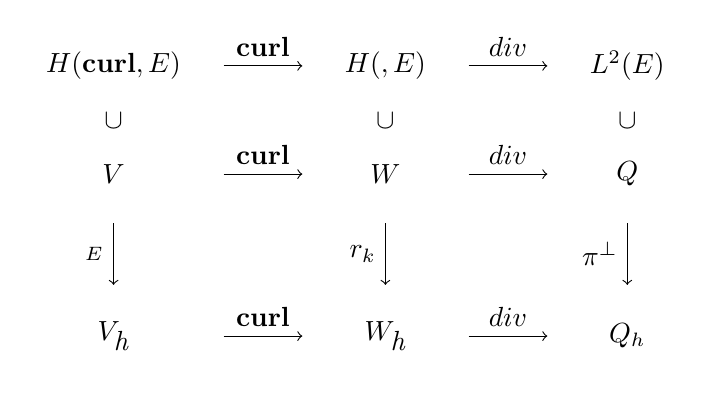
\begin{tikzpicture}[point/.style={circle, inner sep=0pt, minimum size=2pt,fill=red}]
            \matrix[column sep = 1.82mm, row sep = 1.1mm, ampersand replacement = \&] {
             \node {$\text{H}(\textbf{curl},E)$};  
              \& \node (n0) {};
              \& \node      {};
              \& \node (n1) {};
              \& \node (n2) {};
              \& \node {$\text{H}(\Div, E)$}; 
              \& \node (r1c7) {};
              \& \node {};
              \& \node {};
              \& \node (r1c10) {};
              \& \node {$L^2(E)$};\\
             \node (n3) {}; \&\&\&\&\& \node (n5)   {};
              \& \node (r2c7) {};
              \& \node {};
              \& \node {};
              \& \node {};
              \& \node (r2c11) {};\\
             \node (n4) {}; \&\&\&\&\& \node (n6)   {};
              \& \node (r3c7) {};
              \& \node {};
              \& \node {};
              \& \node {};
              \& \node (r3c11) {};\\
             \node (v)  {$V$}; \&\node(fromV){};\&\&\&\node(toW){};\& \node (w) {$W$};
              \& \node (r4c7) {};
              \& \node {};
              \& \node {};
              \& \node (r4c10) {};
              \& \node {$Q$};\\
             \node (n7) {}; \&\&\&\&\& \node (n8)   {};
              \& \node {};
              \& \node {};
              \& \node {};
              \& \node {};
              \& \node (r5c11) {};\\
             \node      {}; \&\&\&\&\& \node        {}; 
              \& \node {};
              \& \node {};
              \& \node {};
              \& \node {};
              \& \node {};\\
             \node      {}; \&\&\&\&\& \node        {}; 
              \& \node {};
              \& \node {};
              \& \node {};
              \& \node {};
              \& \node {};\\
             \node (n11)    {}; \&\&\&\&\& \node (n12) {};
              \& \node {};
              \& \node {};
              \& \node {};
              \& \node {};
              \& \node (r8c11) {};\\
             \node {$V_{\textit{h}} $};                                 
              \& \node (n13) {};
              \& \node       {};
              \& \node (n14) {};
              \& \node (n15) {};
              \& \node {$W_{\textit{h}} $}; 
              \& \node (r9c7) {};
              \& \node {};
              \& \node {};
              \& \node (r9c10) {};
              \& \node {$Q_h$};\\
             };
            \draw[->] (n0) to node[above] {$\textbf{curl}$} (n2); 
            \draw[->] (fromV) to node[above] {$\textbf{curl}$} (toW); 
            \draw[white] (n3) to node {{\color{black}$\cup$}} (n4);
            \draw[white] (n5) to node {{\color{black}$\cup$}} (n6);
            \draw[->] (n7) to node[left] {$\bw_E$} (n11); 
            \draw[->] (n8) to node[left] {$\boldsymbol{r}_k$} (n12); 
            \draw[->] (n13) to node[above] {$\textbf{curl}$} (n15); 
            \draw[->] (r1c7) to node[above] {$\text{div}$} (r1c10);
            \draw[->] (r4c7) to node[above] {$\text{div}$} (r4c10);
            \draw[->] (r9c7) to node[above] {$\text{div}$} (r9c10);
            %\draw[white] (r2c7) to node {{\color{black}$\cup$}} (r3c7);
            \draw[white] (r2c11) to node {{\color{black}$\cup$}} (r3c11);
            \draw[->] (r5c11) to node[left] {$\pi^{\perp}$} (r8c11);
        \end{tikzpicture}
    \end{center}

% subsection definition_of_the_h_div_element (end)

El sigte lema, hacerlo una vez para edge
y una vez para face, para un cierto poliedro, y decir que vale 
la misma cuenta en los otros. Ver (3.79) (3.80) en monk: transf.
de normales y tangentes.\\\\
remite a transform entre prismas etc ... de preliminares\\
\begin{lemma} The edge element interpolators satisfy
\begin{IEEEeqnarray}{rCl}\label{piTransformado}
    \wku(\hat{\bx}) & = & M^{t} \bw_E\bu(F_E(\hat{\bx}))
\end{IEEEeqnarray}
provided $\det M^{t} > 0$.
\end{lemma}
\begin{proof} See Lemmas 5.32 and 5.34 in pages 130 and 131 of~\cite{monk}.  
\end{proof}

% subsection transformaciones_entre_prismas (end)